%!TEX root = ../../exa-ma-d7.1.tex
\section{Software: \Feelpp}
\label{sec:Feelpp:software}

\begin{table}[h!]
    \centering
    { \setlength{\parindent}{0pt}
    \def\arraystretch{1.25}
    \arrayrulecolor{numpexgray}
    {\fontsize{9}{11}\selectfont
    \begin{tabular}{!{\color{numpexgray}\vrule}p{.4\textwidth}!{\color{numpexgray}\vrule}p{.6\textwidth}!{\color{numpexgray}\vrule}}
        \rowcolor{numpexgray}{\rule{0pt}{2.5ex}\color{white}\bf Field} & {\rule{0pt}{2.5ex}\color{white}\bf Details} \\
        \rowcolor{white}\textbf{Consortium} & \begin{tabular}{l}
\Feelpp Consortium\\
\end{tabular} \\
        \rowcolor{numpexlightergray}\textbf{Exa-MA Partners} & \begin{tabular}{l}
CNRS\\
Inria Grenoble\\
Unistra\\
\end{tabular} \\
        \rowcolor{white}\textbf{Contact Emails} & \begin{tabular}{l}
christophe.prudhomme@cemosis.fr\\
vincent.chabannes@cemosis.fr\\
\end{tabular} \\
        \rowcolor{numpexlightergray}\textbf{Supported Architectures} & \begin{tabular}{l}
CPU Only\\
\end{tabular} \\
        \rowcolor{white}\textbf{Repository} & \href{https://github.com/feelpp/feelpp}{https://github.com/feelpp/feelpp} \\
        \rowcolor{numpexlightergray}\textbf{License} & \begin{tabular}{l}
OSS:: GPL v*\\
OSS:: LGPL v*\\
\end{tabular} \\
        \rowcolor{white}\textbf{Bottlenecks roadmap} & \begin{tabular}{l}
B10 - Scientific Productivity\\
B11 - Reproducibility and Replicability of Computation\\
B12 - Pre/Post Processing and In-Situ Processing\\
B2 - Interconnect Technology\\
B6 - Data Management\\
B7 - Exascale Algorithms\\
\end{tabular} \\
        \bottomrule
    \end{tabular}
    }}
    \caption{\Feelpp Information}
\end{table}

\subsection{Software summary}
\label{sec:Feelpp:summary}
\Feelpp is a C++ framework for multiphysics simulations based on the finite element method. 
It is designed to handle complex simulations in a wide variety of fields, including fluid dynamics, electromagnetism, and solid mechanics. 
It focuses on high-performance computing and reproducibility in scientific computation.

\subsection{Purpose}
\label{sec:Feelpp:purpose}
\Feelpp aims to provide a flexible and efficient environment for conducting finite element analysis in multiple scientific domains. 
It allows for the rapid prototyping of numerical models and is built with parallel computing in mind to scale on modern HPC architectures.

\subsection{Programming and Computational Environment}
\label{sec::Feelpp:environment_capabilities}

The following table summarizes these aspects for \Feelpp, providing a view of its programming and computational capabilities.

\begin{table}[h!]
%%    \centering
    {
    \setlength{\parindent}{0pt}
    \def\arraystretch{1.25}
    \arrayrulecolor{numpexgray}
    {\fontsize{9}{11}\selectfont
    \begin{longtable}{lp{.3\textwidth}p{.5\textwidth}}
        \rowcolor{gray}\textbf{\color{white}Category} & \textbf{\color{white}Details} & \textbf{\color{white}Description} \\
        \hline
        \endfirsthead % End of the first head (the header for the first page)
        
        \hline
        \rowcolor{gray}\textbf{Category} & \textbf{Details} & \textbf{Description} \\
        \hline
        \endhead % End of the head (for all other pages)
        
        \hline
        \endfoot % Footer for all but the last page
        
        \hline
        \endlastfoot % Footer for the last page

        \rowcolor{white}Languages  & \begin{tabular}{l}
C++\\
C++17\\
C++20\\
Python\\
\end{tabular} & \Feelpp is primarily developed in C++ and supports modern C++ standards, including C++17 and C++20, which provide enhanced performance, safety features, and modern programming paradigms for high-performance computing applications. This allows \Feelpp to leverage advanced language features such as constexpr, parallel algorithms, and enhanced lambda expressions, improving both code maintainability and computational efficiency. Additionally, \Feelpp integrates with Python, enabling scripting capabilities and facilitating ease of use for rapid prototyping, automation, and integration with scientific workflows. This dual-language support provides flexibility for both performance-critical tasks and user-friendly interfaces. \\
        \rowcolor{numpexlightergray}Parallelism  & \begin{tabular}{l}
MPI\\
Parallelism - C++\\
Task based\\
\end{tabular} & \Feelpp offers robust support for parallel computing, making it suitable for high-performance simulations. It utilizes MPI (Message Passing Interface) for distributed memory parallelism, enabling efficient communication between processes across different nodes in HPC environments. Additionally, \Feelpp implements parallelism directly in C++, allowing fine-grained control over threading and parallel execution within shared memory systems. The framework also supports task-based parallelism thanks to specx, enabling the efficient execution of independent computational tasks, improving load balancing, and optimizing resource usage across heterogeneous computing architectures. This parallelism support ensures scalability and high performance in complex multiphysics simulations.\\
        \rowcolor{white}Data Formats  & \begin{tabular}{l}
Data-management system\\
Ensight\\
Gmsh and associated formats\\
HDF5\\
JSON\\
VTK\\
YAML\\
in-house format\\
\end{tabular} & \Feelpp supports data management, including remote data management systems such as Girder and GitHub. It handles a variety of input and output formats, including Ensight, Gmsh, HDF5, JSON, VTK, YAML, and an in-house format. This flexibility enables \Feelpp to align with the \textbf{FAIR} principles (Findable, Accessible, Interoperable, and Reusable), ensuring efficient data sharing and reuse across different platforms and tools.\\
        \rowcolor{numpexlightergray}Resilience  & \begin{tabular}{l}
Checkpoint restart\\
\end{tabular} & \Feelpp provides resilience support through checkpoint restart functionality. This allows simulations to save their state at specific points, enabling recovery from failures without restarting from the beginning. Binary in-house formats are used for fast restarts, ensuring minimal downtime and efficient continuation of long-running computations, especially on large-scale HPC systems.\\
        \rowcolor{white}DevOps & \begin{tabular}{l}
Continuous Benchmarking\\
Continuous Delivery\\
Continuous Integration\\
\end{tabular} & Outlines the development and operational practices including continuous integration, containerization, and testing methodologies.  \\
        \rowcolor{numpexlightergray}Packaging  & \begin{tabular}{l}
Debian\\
Fedora\\
Spack\\
Ubuntu\\
\end{tabular} & \Feelpp is available in various packaging formats to ensure broad compatibility across different platforms. It is packaged for popular Linux distributions and HPC environments, with specific mirrors and repositories:\\
        \rowcolor{white}Testing  & \begin{tabular}{l}
Unit\\
Validation\\
Verification\\
\end{tabular} & Testing methodologies employed to ensure software quality and correctness.\\
        \rowcolor{numpexlightergray}Containerization  & \begin{tabular}{l}
Docker\\
Singularity\\
\end{tabular} & Container technologies used to package and deploy the software.\\
        \rowcolor{white}Interfaces  & \begin{tabular}{l}
Dymola/OpenModelica/FMU\\
HPdomain decomposition methods\\
MMG/ParMMG\\
OpenTurns\\
PETSc\\
Salome\\
\end{tabular} & List of software \Feelpp has interfaces with.\\
        \bottomrule
    \end{longtable}
    }}
    \caption{\Feelpp programming and computational environment}
\end{table}

            {\fontsize{9}{11}\selectfont
\begin{longtable}{lp{0.3\textwidth}p{0.5\textwidth}}
        \caption{\Feelpp programming and computational environment}\label{tab:Feelpp:environment_capabilities} \\
        \rowcolor{gray}\textbf{\color{white}Category} & \textbf{\color{white}Details} & \textbf{\color{white}Description} \\
        \hline
        \endfirsthead % End of the first head (the header for the first page)
        
        \hline
        \rowcolor{gray}\textbf{\color{white}Category} & \textbf{\color{white}Details} & \textbf{\color{white}Description} \\
        \hline
        \endhead % End of the head (for all other pages)
        
        \hline
        \endfoot % Footer for all but the last page
        
        \hline
        \endlastfoot % Footer for the last page
    
        \rowcolor{white}Languages  & \begin{tabular}{l}
                C++\\
                C++17\\
                C++20\\
                Python\\
                \end{tabular} & \Feelpp is primarily developed in C++ and supports modern C++ standards, including C++17 and C++20, which provide enhanced performance and safety features for high-performance computing applications. It also integrates with Python for scripting capabilities. \\
        
        \rowcolor{numpexlightergray}Parallelism  & \begin{tabular}{l}
                MPI\\
                Parallelism - C++\\
                Task based\\
                \end{tabular} & \Feelpp offers robust support for parallel computing, utilizing MPI for distributed memory parallelism and implementing task-based parallelism to improve load balancing and resource usage. \\
        
        \rowcolor{white}Data Formats  & \begin{tabular}{l}
                Data-management system\\
                Ensight\\
                Gmsh and associated formats\\
                HDF5\\
                JSON\\
                VTK\\
                YAML\\
                in-house format\\
                \end{tabular} & \Feelpp supports various data formats for efficient data sharing and reuse, aligning with the FAIR principles. \\
        
        \rowcolor{numpexlightergray}Resilience  & Checkpoint restart & \Feelpp provides resilience support through checkpoint restart functionality. This allows simulations to save their state at specific points, enabling recovery from failures without restarting from the beginning. Binary in-house formats are used for fast restarts, ensuring minimal downtime and efficient continuation of long-running computations, especially on large-scale HPC systems.\\
        
        \rowcolor{white}DevOps & \begin{tabular}{l} Continuous Benchmarking\\
                Continuous Delivery\\
                Continuous Integration\\
                \end{tabular} & \Feelpp is developped on GitHub and uses GitHub Actions workflows to ensure the quality of the developments. The main branch is protected and only accepted reviewed PR can be merged. \Feelpp is not only rebuilt by the CI but also tests are run.  Upon merge, a packaging workflow is trigerred to generate Debian-based packages as well as Docker and Apptainer images. Once Apptainer images are available, benchmarks are trigerred on super computer to check the performances, see~\cref{feelpp-ci} and~\cref{feelpp-cb} for a graphical representation.\\ 
        
        \rowcolor{numpexlightergray}Packaging  & Debian, Fedora, Spack, Ubuntu & Debian-based systems: Available via the APT repository at \href{https://apt.feelpp.org}{apt.feelpp.org}. Detailed installation instructions can be found in the documentation: \href{https://docs.feelpp.org/user/latest/install/index.html}{\Feelpp Installation Guide}.
        Fedora: Distributed via Docker images, simplifying deployment in containerized environments.
        Spack: Supported by Spack for high-performance computing environments, with a mirror available at \href{https://ghcr.io/feelpp/spack}{ghcr.io/feelpp/spack}.
        Ubuntu: Also available through the same APT repository for Debian-based systems.\\

        \rowcolor{white}Testing  & \begin{tabular}{l}
                Unit\\
                Validation\\
                Verification\\
                \end{tabular} & \Feelpp includes a comprehensive suite of nearly 1,000 tests executed via ctest. These tests correspond to applications run both sequentially and in parallel. In most cases, applications are tested in both modes; only on very rare occasions are they run exclusively in either sequential or parallel mode. Each application contains numerous tests that perform unit testing or verify expected mathematical properties. To detect excessive execution time regressions, timeouts are configured for the tests. Finally, some tests are mini-applications or benchmarks that perform verification or validation against reference results.\\        

        \rowcolor{numpexlightergray}Containerization  & Docker, Singularity & \Feelpp supports Docker and Apptainer/Singularity containers built either from source or from Debian-based packages. Both container type images are stored on \url{https://ghcr.io/feelpp/feelpp}. Images with tags containing \texttt{-sif} appended are apptainer images, the other ones are docker images. \\
        
        \rowcolor{white}Interfaces  &\begin{tabular}{l}
                Dymola/OpenModelica/FMU\\
                hpddm\\
                MMG/ParMMG\\
                OpenTurns\\
                PETSc\\
                Salome\\
                CGAL\\
                Scimba
                \end{tabular} & \Feelpp can easily be interfaced with various software thanks to the use of standard open formats and a flexible \Cpp design.\\

               
    \end{longtable}
    }



    The figure~\cref{fig:feelpp-ci} shows the \Feelpp Continuous Integration Workflow using GitHub Actions.
    \begin{figure}
        \centering
        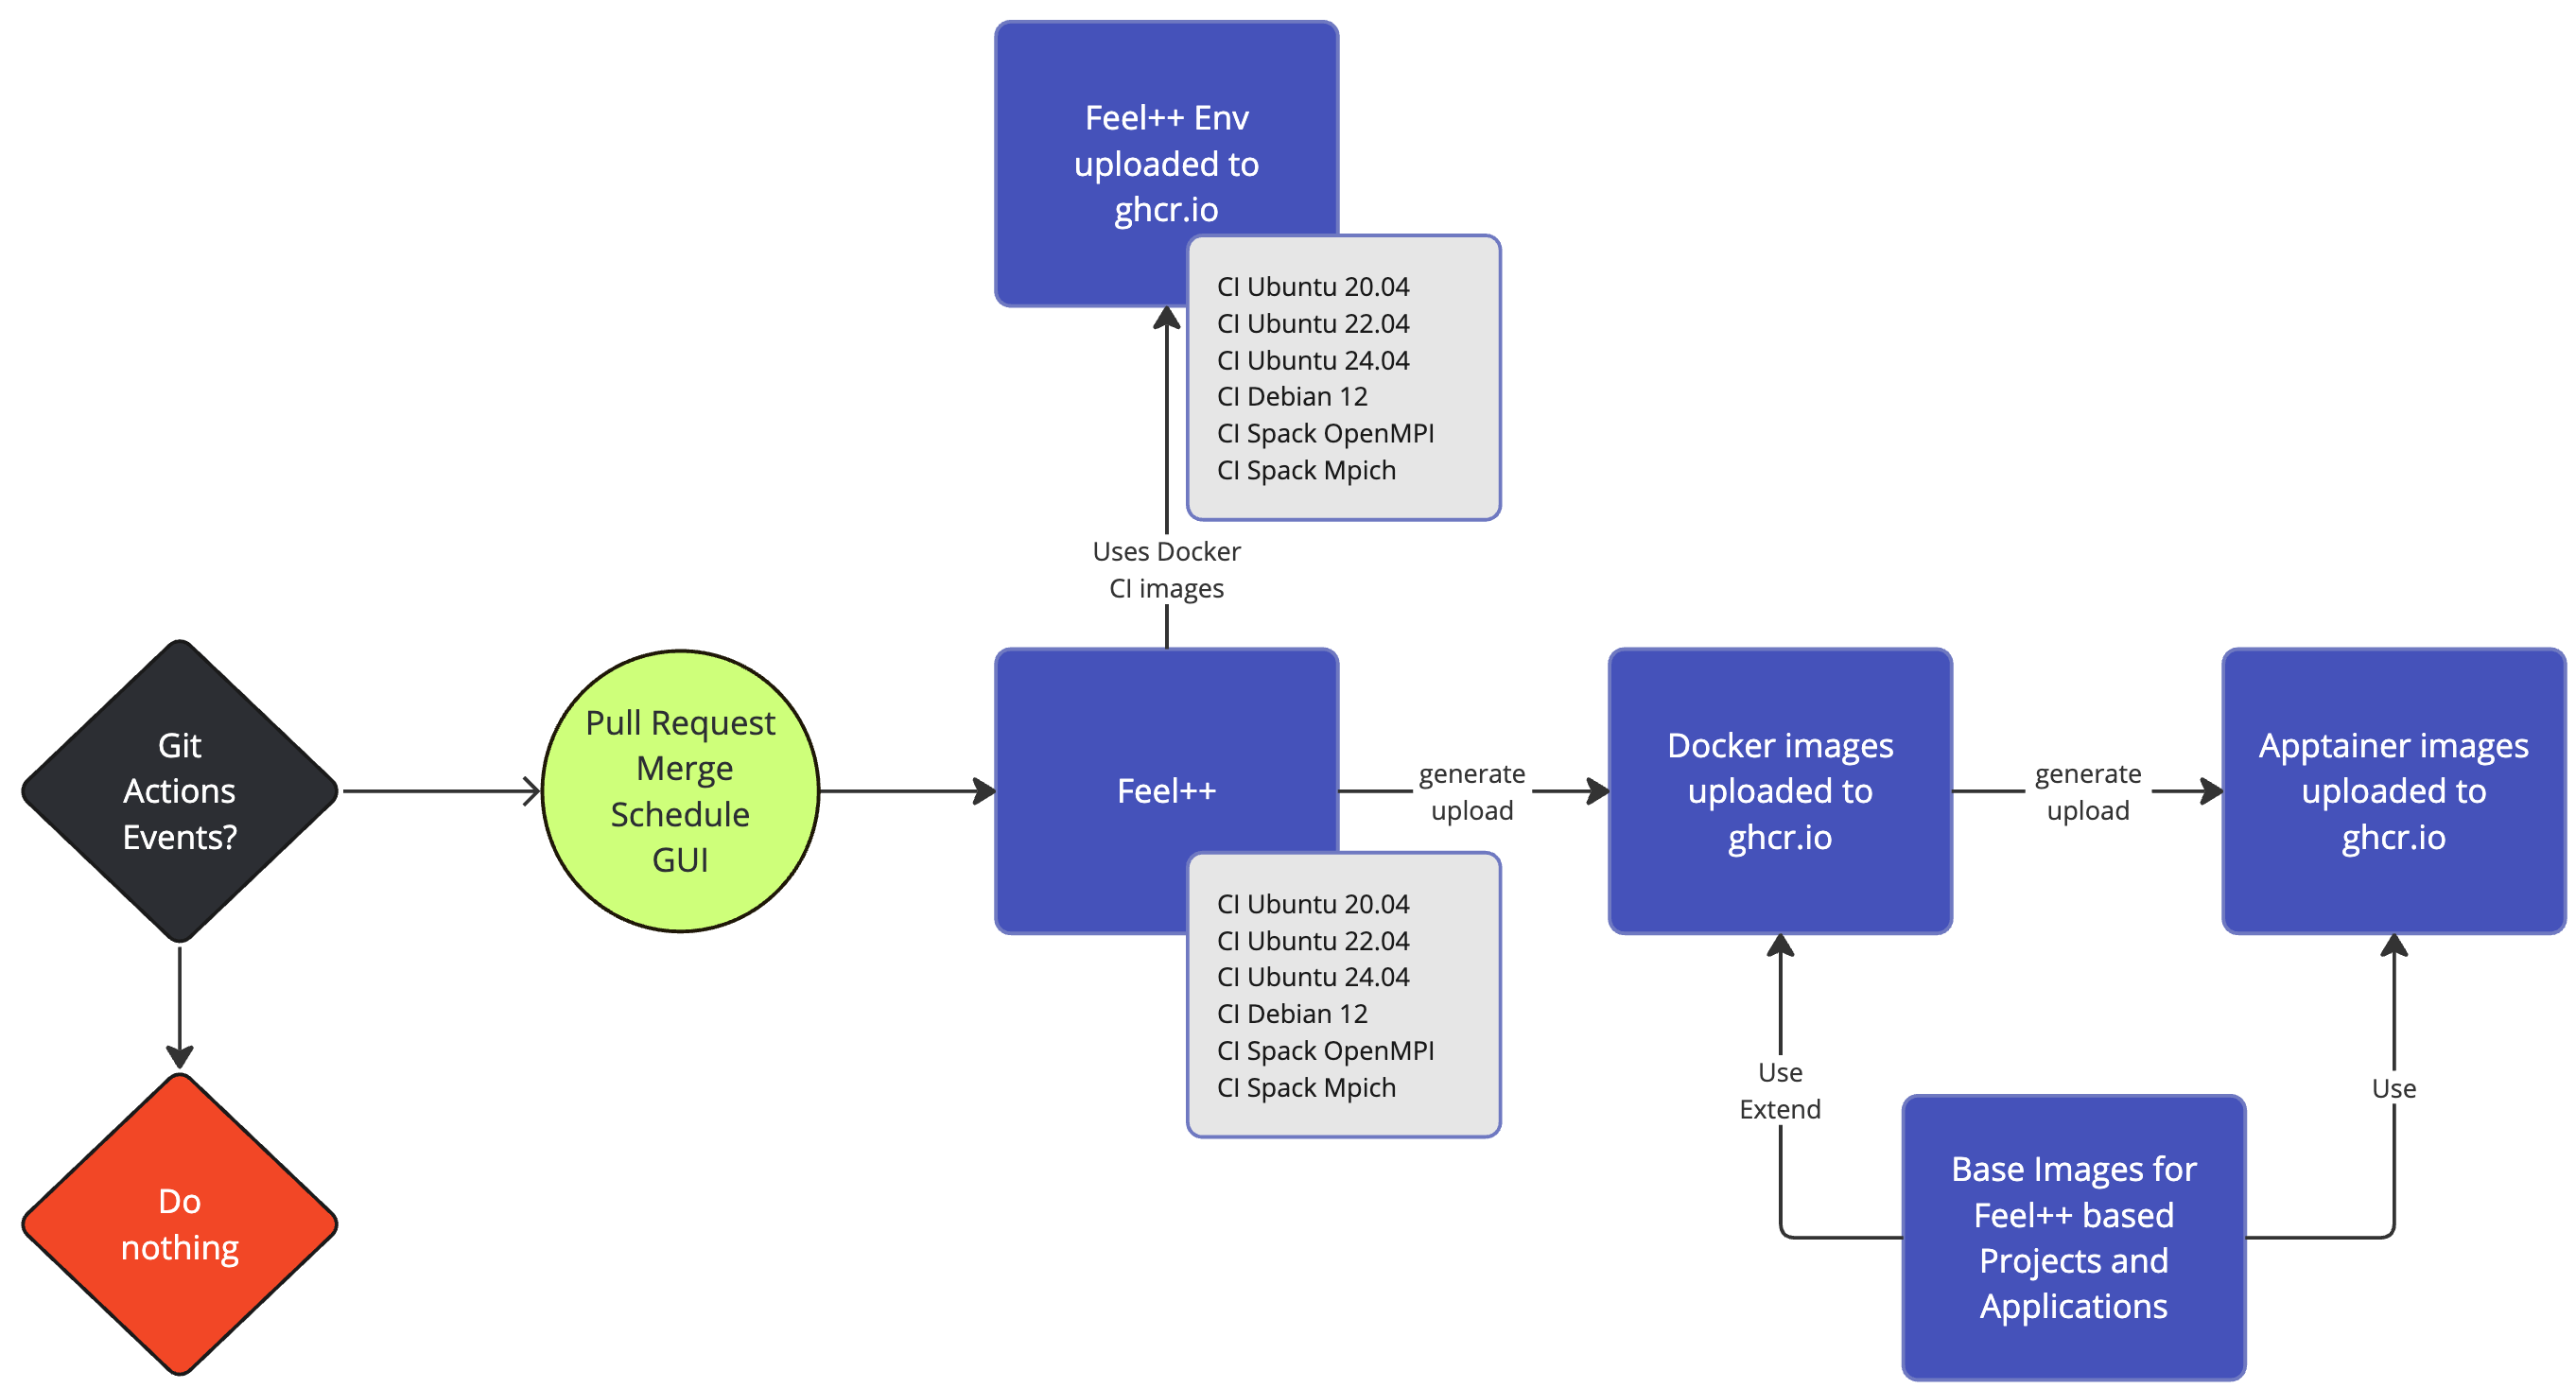
\includegraphics[width=0.8\textwidth]{graphics/feelpp/feelpp-ci-workflow.png}
        \caption{\Feelpp Continuous Integration Workflow using GitHub Actions}
        \label{fig:feelpp-ci}
    \end{figure}

    The figure~\cref{fig:feelpp-cb} shows the \Feelpp Continuous Benchmarking Workflow using GitHub Actions and Reframe which is quite close to the methodology described in~\cref{sec:methodology-regression-reframe}.
    \begin{figure}
        \centering
        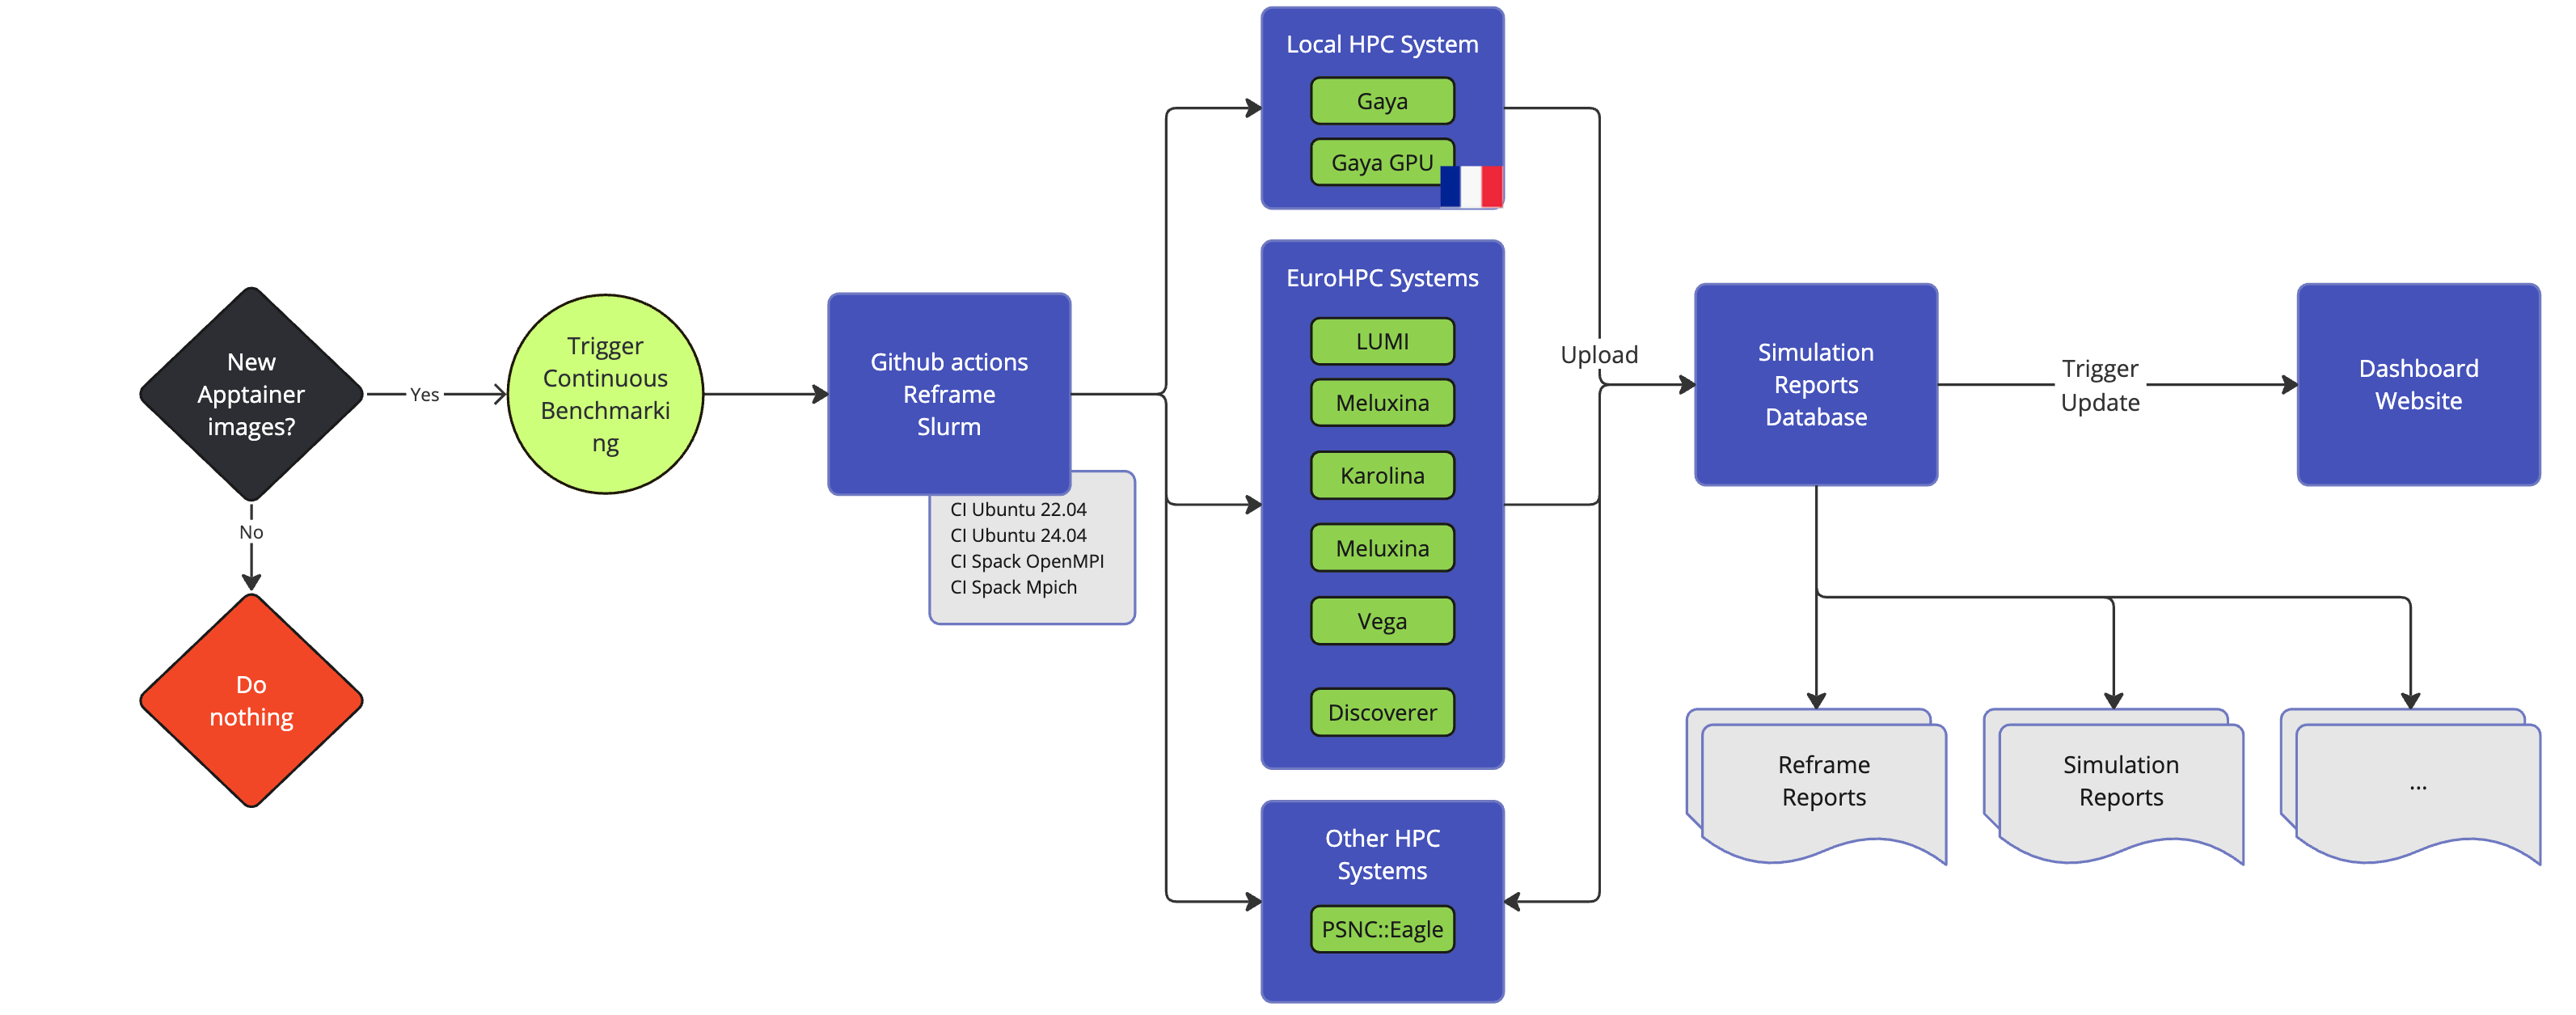
\includegraphics[width=0.8\textwidth]{graphics/feelpp/feelpp-cb-workflow.png}
        \caption{\Feelpp Continuous Benchmarking Workflow using GitHub Actions and Reframe}
        \label{fig:feelpp-cb}
    \end{figure}

\subsection{Mathematics}
\label{sec:Feelpp:mathematics}
\Feelpp is based on the finite element method (FEM), which is used for solving partial differential equations (PDEs) in complex geometries. 
It leverages advanced numerical techniques to ensure accuracy and scalability, including adaptive mesh refinement, domain decomposition, and error estimation.

\subsection{Relevant Publications}
\label{sec:Feelpp:publications}
Relevant publications include:
\begin{itemize}
    \item \fullcite{prudhomme_feelppfeelpp_2024} is the last preview of the \Feelpp software. The documentation is available online at \url{https://docs.feelpp.org}.
    \item \fullcite{saigre_model_2024} 
    \item \fullcite{van_landeghem_mathematical_2024}
    \item \fullcite{prudhomme_ktirio_2024}
\end{itemize}

\subsection{Acknowledgements}
\label{sec::Feelpp:acknowledgements}
The software has been developed with the support of the following funding agencies and institutions through various research projects: 
\begin{itemize}
   \item Université de Strasbourg
   \item CNRS
   \item ANR
   \item Région Grand Est
   \item AMIES
   \item European Commission
   \item EuroHPC JU
\end{itemize}
